\documentclass{oblivoir}
\usepackage{amsmath,amssymb,amsthm,kotex,mdframed,paralist,chngcntr}
\usepackage{kswrapfig}

\newcounter{num}
%\newcommand{\defi}[1]
%{\bigskip\noindent\refstepcounter{num}\textbf{정의 \arabic{num}) #1}\par}
%\newcommand{\theo}[1]
%{\bigskip\noindent\refstepcounter{num}\textbf{정리 \arabic{num}) #1}\par}
%\newcommand{\exam}[1]
%{\bigskip\noindent\refstepcounter{num}\textbf{예시 \arabic{num}) #1}\par}
\newcommand{\prob}[1]
{\bigskip\noindent\refstepcounter{num}\textbf{문제 \arabic{num}) #1}\par}
%\newcommand{\howo}[1]
%{\bigskip\noindent\refstepcounter{num}\textbf{숙제 \arabic{num}) #1}\par\bigskip}

\newcommand{\ans}{{\raggedleft\textbf{답 : (\qquad\qquad\qquad\qquad\qquad\qquad)}
\par}}

\renewcommand{\proofname}{증명)}
\counterwithout{subsection}{section}


%%%
\begin{document}
\Large

\title{승재 03 - 최고수준 수학}
\author{}
\date{\today}
\maketitle
%\tableofcontents

\newpage

%
\prob{p95, \#4-1-1}
\kswrapfig[Pos=r]{09541-1}{
오른쪽은 반지름이 10cm인 원의 일부분 안에 지름이 10cm인 반원 2개를 그린 것입니다.
색칠한 부분의 둘레는 몇 cm입니까?(원주율 : 3)

\ans{}
}
%

%
\prob{p95, \#4-1-2}
\kswrapfig[Pos=r]{09541-2}{
오른쪽은 한 변의 길이가 20cm인 정사각형 안에 반지름이 20cm인 원의 일부분과 지름이 20cm인 반원 2개를 그린 것입니다.
색칠한 부분의 둘레는 몇 cm입니까?(원주율 : 3)

\ans{}
}
%


\newpage

%
\prob{p95, \#4-1-3}
아래 그림은 반지름이 20cm인 원의 일부분 안에 지름이 20cm인 반원 2개를 그린 것입니다.
색칠한 부분의 둘레는 몇 cm입니까?(원주율 : 3)
\begin{figure}[h]
\centering
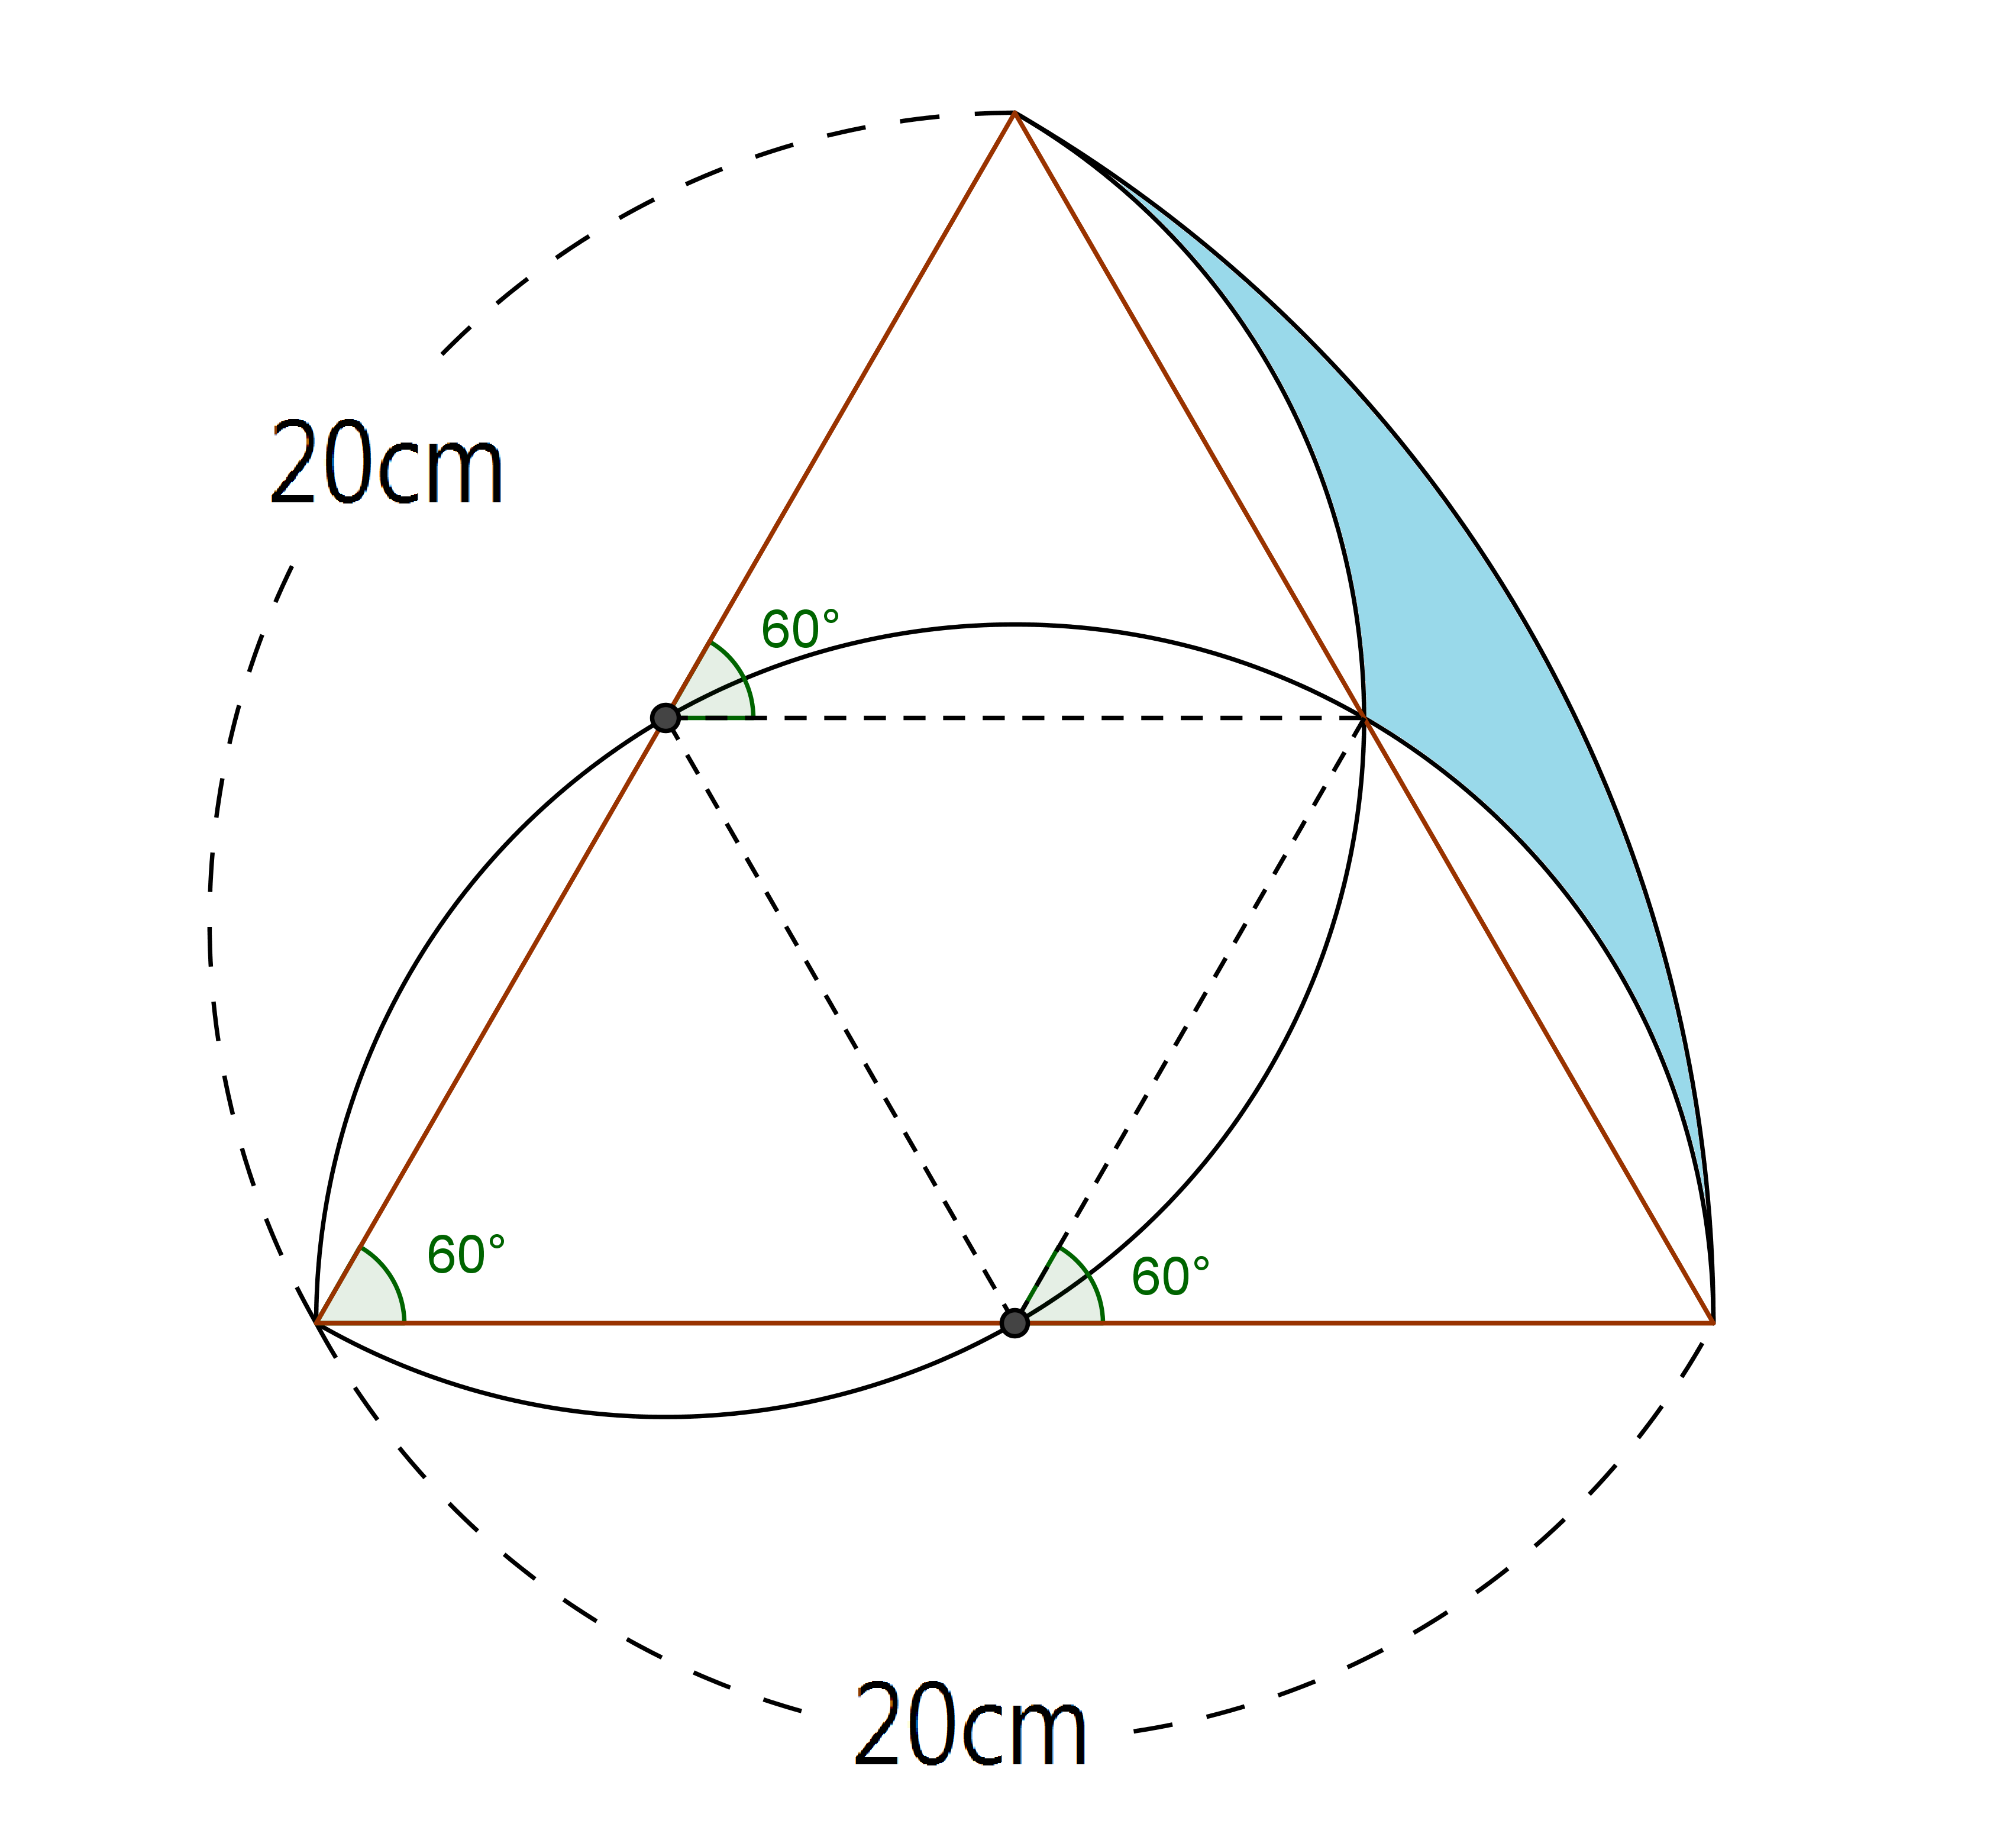
\includegraphics[width=0.7\textwidth]{09541-3}
\end{figure}

\ans{}
%

\newpage

%
\prob{p101, \#11-1}
\kswrapfig[Pos=r]{10111-1}{
오른쪽 도형은 지름이 10cm인 반원을 점 ㄴ을 중심으로 \(45^\circ\)만큼 회전시킨 것입니다.
색칠한 부분의 넓이는 몇 cm\(^2\)입니까?
(원주율 : 3)

\ans{}
}
%

%
\prob{p101, \#11-2}
\kswrapfig[Pos=r]{10111-2}{
오른쪽 도형은 지름이 10cm인 반원을 점 ㄴ을 중심으로 \(90^\circ\)만큼 회전시킨 것입니다.
색칠한 부분의 넓이는 몇 cm\(^2\)입니까?
(원주율 : 3)

\ans{}
}
%
\end{document}